%%%%%%%%%%%%%%%%%%%%%%%%%%%%%%%%%%%%%%%
%%% LATEX HEADERS
%%%%%%%%%%%%%%%%%%%%%%%%%%%%%%%%%%%%%%%

\documentclass[article]{JSSstyle/jss}
\usepackage{rotating}                           
\usepackage[dvips]{epsfig}
\usepackage{multirow}
\usepackage{amsfonts,amssymb,amsmath}
\usepackage{array}                      
\usepackage{url}
\usepackage{thumbpdf}
\usepackage{natbib}

\usepackage{vmargin}
    \setpapersize{USletter}
    \setmarginsrb{1.0in}{1.0in}{1.0in}{1.0in}{0.5in}{0.2in}{0in}{0.2in}
\renewcommand{\baselinestretch}{1.25}

%%%%%%%%%%%%%%%%%%%%%%%%%%%%%%%%%%%%%%%
%%% SHORTCUTS
%%%%%%%%%%%%%%%%%%%%%%%%%%%%%%%%%%%%%%%

% open office tricks
\newcommand\textsubscript[1]{\ensuremath{{}_{\text{#1}}}}

%%%%%%%
%%% Vignette Headers
%%%%%%%

%\VignetteIndexEntry{bard}
%\VignetteKeywords{automated redistricting}
%\VignetteVersion{1.0}
%\VignetteTitle{Better Autometed redistricting} 

%%%%%%%%%%%%%%%%%%%%%%%%%%%%%%%%%%%%%%%
%%% DOCUMENT HEADERS
%%%%%%%%%%%%%%%%%%%%%%%%%%%%%%%%%%%%%%%

\author{Micah Altman\\Harvard University
\And Michael P. McDonald \\George Mason University\\Brookings Institution
}
\Plainauthor{Micah Altman, Michael P. McDonald}
\title{\pkg{BARD}: Better Automated Redistricting}
\Plaintitle{BARD: Better Automated Redistricting}
\Shorttitle{\pkg{Better Automated Redistricting}}
\Keywords{redistricting, optimization}

\Address{
Micah Altman\\
Senior Research Scientist\\
Institute for Quantitative Social Science\\
Harvard University\\
1737 Cambridge Street, Room 325\\ 
Cambridge, MA, 02138.\\
United States of America\\
E-mail: \email{micah\_altman@harvard.edu}\\
URL: \url{http://www.hmdc.harvard.edu/micah_altman/}\\
\\
Michael P. McDonald\\
Associate Professor, Department of Public and International Affairs\\
George Mason University\\
4400 University Drive - 3F4\\
Fairfax, VA 22030-4444 \\
E-mail: \email{mmcdon@gmu.edu}\\
URL: \url{http://elections.gmu.edu/}\\
}

\Abstract{
BARD provides a set of open source tools to automatically create and
analyze redistricting plans. These tools support both scientific analysis
of existing redistricting plans and citizen participation in creating new plans.
}

%%% Below is a magic header line, with two %:
%% need no \usepackage{Sweave.sty}
    
%%%%%%%%%%%%%%%%%%%%%%%%%%%%%%%%%%%%%%%
%%% DOCUMENT STARTS
%%%%%%%%%%%%%%%%%%%%%%%%%%%%%%%%%%%%%%%

\begin{document}

\section{Introduction - Automated Redistricting for Political Participation and Analysis}

Legislative redistricting is among the most politically charged 
tasks in American politics.  District lines affect which political 
party wins control of a legislative body, the reelection success of 
incumbents, and election of minority preferred candidates.  A recent United States 
Supreme Court case, \emph{LULAC} v. \emph{Perry} [547 U.S. 2006], is instructional of the political consequences of redistricting.  The Court 
upheld parts of a controversial 2003 Texas congressional redistricting 
plan that promoted the election of Republicans at the cost of 
incumbent Democrats, but struck down districts in the southern part 
of the state that disadvantaged the election of minority candidates 
of choice.  The ruling capped a series of sometimes bizarre events 
that included the state legislature's closure when members fled the 
state and the downfall of a powerful congressional leader due to 
related campaign finance violations.

In the 1960s, scholars envisioned taking politics out of 
redistricting by automatically drawing districts using computer programs \citep[][]{Vickrey61, WeaverHess63}.  After 
all, at its most basic level, redistricting can be reduced to a simply stated
(albeit computationally difficult) mathematical partitioning problem.  These scholars 
reasoned that an algorithm following neutral criteria would draw 
districts blind to politics.  Programs were indeed developed, 
however, they fell short of practical use.  The problem turned out 
to be more computationally intensive than anticipated.  The seemingly straight-forward mathematical operationalization 
of common redistricting goals became a debate subject as implementation of criteria is often percevied to have partisan consequences.  
Even today, the best commercially available software cannot 
automatically draw congressional or state legislative districts that 
would pass federal or state constitutional muster. 

Redistricting's complexity has frozen out the public from the 
redistricting process.  Only well-funded political organizations are capable 
of putting together the data, equipment, and expertise needed to 
conduct a statewide redistricting.  Thus, a conflict of interest 
develops at the expense of the public good.  While some states have 
attempted redistricting reform \citep[][]{McDonald06}, in most 
states the people who are draw the lines are the same people affected by them.

We are now revisiting advocates' aspirations automated redistricting software.  
Processing power has increased tremendously even while price has 
decreased, data are now easily assessible on the internet, new
optimization heuristics have emerged, and the flourishing
open source programming community has facilitated
new approaches to the automated redistricting problem. We are developing 
just such a program.  Our program accepts a draft plan, either supplied by a user or generated randomly by one of several algorithms.  The program then employs metaheuristics to improve the plan on several 
goals such as minimizing political bias, maximizing the 
number of competitive districts, or aligning districts with local political or community 
boundaries. Although the computational problem is too difficult
to ensure that the resulting plan is \emph{optimal}, it may yield a useful
improvement over the starting map and may enable public interest groups to generate viable plans. 

While a computer program like this would be a powerful counterbalance to entrenched political interests, it would be also of scholarly and legal interest by providing a powerful way to 
explore the effects of redistricting goals and constraints. By taking  
existing, proposed, and automatically generated hypothetical plans, 
and then having the computer adjust them to fit the 
proposed redistricting rules, we are able to systematically 
examine the effects such rules have and the tradeoffs 
those rules impose among competing redistricting goals. 
This methodology has long been used in the U.K. in the field of political 
geography, but with rare exceptions has not been applied to U.S. 
elections, in part because of the computational difficulties 
involved in applying this method to large districting problems. Furthermore, 
by taking an existing plan and adjusting it to better meet a
desired goal, we can explore the tradeoffs between that goal and other characteristics of 
the plan.  In many cases, this even yields a window into the intent 
of the original plans author. 

We call our computer program BARD for \textbf{B}etter \textbf{A}utomated 
\textbf{R}e\textbf{D}istricting.\footnote{Tolkein fans will also recognize the 
reference to the slayer of the dragon Smaug, perhaps the most 
terrible of salamanders.} The program contains a set of open source software (licensed under the GPL)
tools to automatically create and analyze redistricting plans. These 
tools support both scientific analysis of existing redistricting 
plans and citizen participation in creating new plans.

\section{A Mathematical Formulation of Redistricting Criteria}

When redistricting authorities draw district boundaries they do not 
simply take pen to paper.  They also analyze information associated with the geographic components of districts to ensure that maps satisfy legal requirements. 
To solve redistricting problems with a computer, we must formalize the general analogous mathematical problem.  Since redistricting 
intrinsically involves assigning discrete blocks of geography (or 
discrete individuals) to districts to achieve a set of goals that is a function 
of the redistricting plan as a whole, the corresponding mathematical 
problem falls into the general area of combinatoric optimization. 

Perhaps among the most important criterion is that districts 
must have equal population,\footnote{Congressional districts must be 
of less than a one percent population division to ensure that they 
conform to legal standards.  State legislative districts are 
permitted a ten percent population deviation under federal law, 
though some state laws require less deviation \citep[][]{CainMacMc05}
.} and the way the U.S. Census Bureau releases population data further guides how the redistricting problem is formalized.  These data are not reported for individuals, rather, to protect the 
confidentiality of respondents, data are 
aggregated into discrete geographic entities known as census 
``blocks'' which roughly conform to a city block in urban areas.  It is not difficult to imagine census blocks as corresponding to a 
points on a graph.  Indeed, Geographic Information Systems (GIS) 
programs plot the vertices of census blocks (and higher geographic 
units, such as counties and cities) onto a screen for user 
manipulation.  GIS redistricting modules enable users to assign blocks to districts through simple 
point and click operations.

Characteristic data associated with each block can be displayed 
on screen.  For example, in the case of equal population 
requirements, blocks can be associated with their total population.  
If a district needs more population, a user can click on blocks 
adjacent to a district to identify those that will help meet a 
target population number.  GIS programs are well-suited to display 
and produce summary statistics of similar data, such as racial 
population data, which are used to meet target racial population 
numbers to conform with the Voting Rights Act, and election data, 
which are used to predict political outcomes.  Indeed, we might think 
of all such characteristic block data as belonging to the same 
family for optimization purposes.

Another important criterion is that districts must (usually) be contiguous, or 
connect.\footnote{While this is  a legal requirement in many states, it is
not a Federal requirement. And there 
are documented instances of non-contiguous districts or districts of 
questionable contiguity because they are connected over water 
without a bridge \citep[][]{Altman98}.  For example, Wisconsin 
requires districts to be composed entirely of wards which are 
sometimes non-contiguous when odd city boundaries create islands of 
incorporated or unincorporated territory.  The 61\textsuperscript{st} Assembly district created in 2001 is non-contiguous 
as a result of containing such a ward on its perimeter.  To 
avoid having non-contiguous districts, the state created a legal 
fiction by stating that all wards are contiguous, see Wisconsin Code 5.15(1)(b)}   
Geospatial coordinate data used to plot census blocks can also be used to determine if two 
blocks are connected to one another.  (In normal operation,
the boundaries of the blocks are used to generate a complete contiguity matrix that  
lists every blocks's neighbors and thus can be used to quickly determine if 
a proposed plan satisfies contiguity.)

Another quasi-geographic set of criteria that are often found in state law is  
`respect' for geographic or political features such as city or county 
boundaries, communities of interest (often defined by redistricting 
authorities), or other `natural'  features such as rivers or mountain ranges.  Capturing  these criteria mathematically is simple: any set 
of census blocks can be defined as belonging to a grouping set and
a penalty for splitting groups can be added to the overall rule for evaluating (scoring) a redistricting plan.
(We are sympathetic to the argument put forth by Forest \citep[][]{Forest04} 
that using only quantitative data to represent communities of interest can result
in `thin' representations of community. Using the technique just described, the BARD system can incorporate
information about the boundaried of communities of interest based on external qualitative analysis and ``thick'' descriptions.) 
An example of this type of community cost function is included in the BARD package.  
The twist is that these criteria are often secondary to equal 
population, contiguity, and Voting Rights concerns, and so the scores
associated with each criterion needs to be properly weighted, in order to
 permit some violation of feature boundaries to 
accommodate superseding criteria.

\section{Improving Algorithms for Automated Redistricting} 

Within the general combinatoric optimization framework are many 
ways to represent particular redistricting problems 
mathematically \citep[see][]{Altman97}. However, representing 
redistricting as a \emph{graph partitioning} problem is the most 
natural formulation, since it allows the expression of geographic 
values, such as compactness and contiguity in a simple and direct 
way. Furthermore, in previous research (below), this representation 
seems to be the most amenable to an efficient solution. 
\footnote{Less commonly, set-partitioning and integer programming 
approaches have been used to solve the redistricting problem. These 
are mathematically equivalent, although incorporating contiguity 
requires that a large number of side constraints be enumerated in 
formulating each problem instance. Geographic site-selection and 
facility allocation problems, as found in the operations research 
literature, are related to the redistricting problem but no 
techniques are available currently to reformulate arbitrary 
redistricting problems in these terms.  In terms of fundamental 
computational complexity, the particular problem representation is 
less important, since one could convert a redistricting problem 
instance back and forth among any different NP-complete problem 
representation in polynomial time. However, in practice, a proper 
choice of representation can make it much easier to formulate and 
solve the problem.}  

To put the problem in formal terms:

%TODO: Fix subscripts

\begin{enumerate}
\item Let \textbf{x}\textit{\textsubscript{i}} refer to the
\textit{i}\textsuperscript{th} census block, $\textit{x}\textit{\textsubscript{i}}\in{\textbf{X}}$ 
where \textbf{X} is the set of all census blocks in a jurisdiction. These blocks are
vector{}-valued, and we will assume that blocks are associated to various
population values, partisan registration percentages, and geographic
locations, among other features.
\textbf{d}\textit{\textsubscript{i}} refers to the
\textit{i}\textsuperscript{th} district. \ A district is a set of
census blocks: % MathType!MTEF!2!1!+-
% feqaeaartrvr0aaatCvAUfeBSjuyZL2yd9gzLbvyNv2CaerbuLwBLn
% hiov2DGi1BTfMBaeXatLxBI9gBaebbnrfifHhDYfgasaacH8srps0l
% bbf9q8WrFfeuY-Hhbbf9v8qqaqFr0xc9pk0xbba9q8WqFfea0-yr0R
% Yxir-Jbba9q8aq0-yq-He9q8qqQ8frFve9Fve9Ff0dmeaabaqaciGa
% caGaaeqabaaaamaaaOqaaiaahsgadaWgaaWcbaGaamyAaaqabaGccq
% GH9aqpdaGadaqaaiaahIhadaqhaaWcbaGaamOAaaqaaaaakiaabYca
% caWH4bWaa0baaSqaaiaadUgaaeaaaaGccaqGSaGaaeOlaiaab6caca
% qGUaGaaeilaiaahIhadaqhaaWcbaGaamOBaaqaaaaaaOGaay5Eaiaa
% w2haaaaa!4186!
\[
{\bf d}_i  = \left\{ {{\bf x}_j^{} {\rm ,}{\bf x}_k^{} {\rm ,}...{\rm ,}{\bf x}_n^{} } \right\}
\]
\item 
\textbf{p}\textit{\textsubscript{i}} refers to a particular plan. A plan
is a partition of the set of all census blocks \textbf{X} into a disjoint set of districts, such that $\textbf{X}=\bigcup{\textbf{d}\textit{\textsubscript{i}}}$ and $\emptyset=\bigcap{\textbf{d}\textit{\textsubscript{i}}}$:\footnote{A small number of jurisdictions permit 
overlapping ``floterial'' districts, which permit the assignment of census blocks to more than one district.  We have not implemented a metaheuristic
optimization algorithm for floterial districts.}
% MathType!MTEF!2!1!+-
% feqaeaartrvr0aaatCvAUfeBSjuyZL2yd9gzLbvyNv2CaerbuLwBLn
% hiov2DGi1BTfMBaeXatLxBI9gBaebbnrfifHhDYfgasaacH8srps0l
% bbf9q8WrFfeuY-Hhbbf9v8qqaqFr0xc9pk0xbba9q8WqFfea0-yr0R
% Yxir-Jbba9q8aq0-yq-He9q8qqQ8frFve9Fve9Ff0dmeaabaqaciGa
% caGaaeqabaaaamaaaOqaaiaahchadaWgaaWcbaGaamyAaaqabaGccq
% GH9aqpdaGadaqaaiaahsgadaqhaaWcbaGaamymaaqaaaaakiaabYca
% caqGUaGaaeOlaiaab6cacaqGSaGaaCizamaaDaaaleaacaWGUbaaba
% aaaaGccaGL7bGaayzFaaaaaa!3E5A!
\[
{\bf p}_i  = \left\{ {{\bf d}_1^{} {\rm ,}...{\rm ,}{\bf d}_n^{} } \right\}
\]
\item 
\textbf{G = (V,}\textbf{\textit{E}}\textbf{)} \textmd{is a mathematical
graph representing the underlying census block geography. Each} node
\textbf{v}\textit{\textsubscript{i}} in g represents a census block,
and each edge \textbf{e}\textit{\textsubscript{i,j}} denotes physical
adjacency of those block
\end{enumerate}

Figure 1 provides a graphical illustration: 

\begin{figure}[!b]
  \begin{center}
    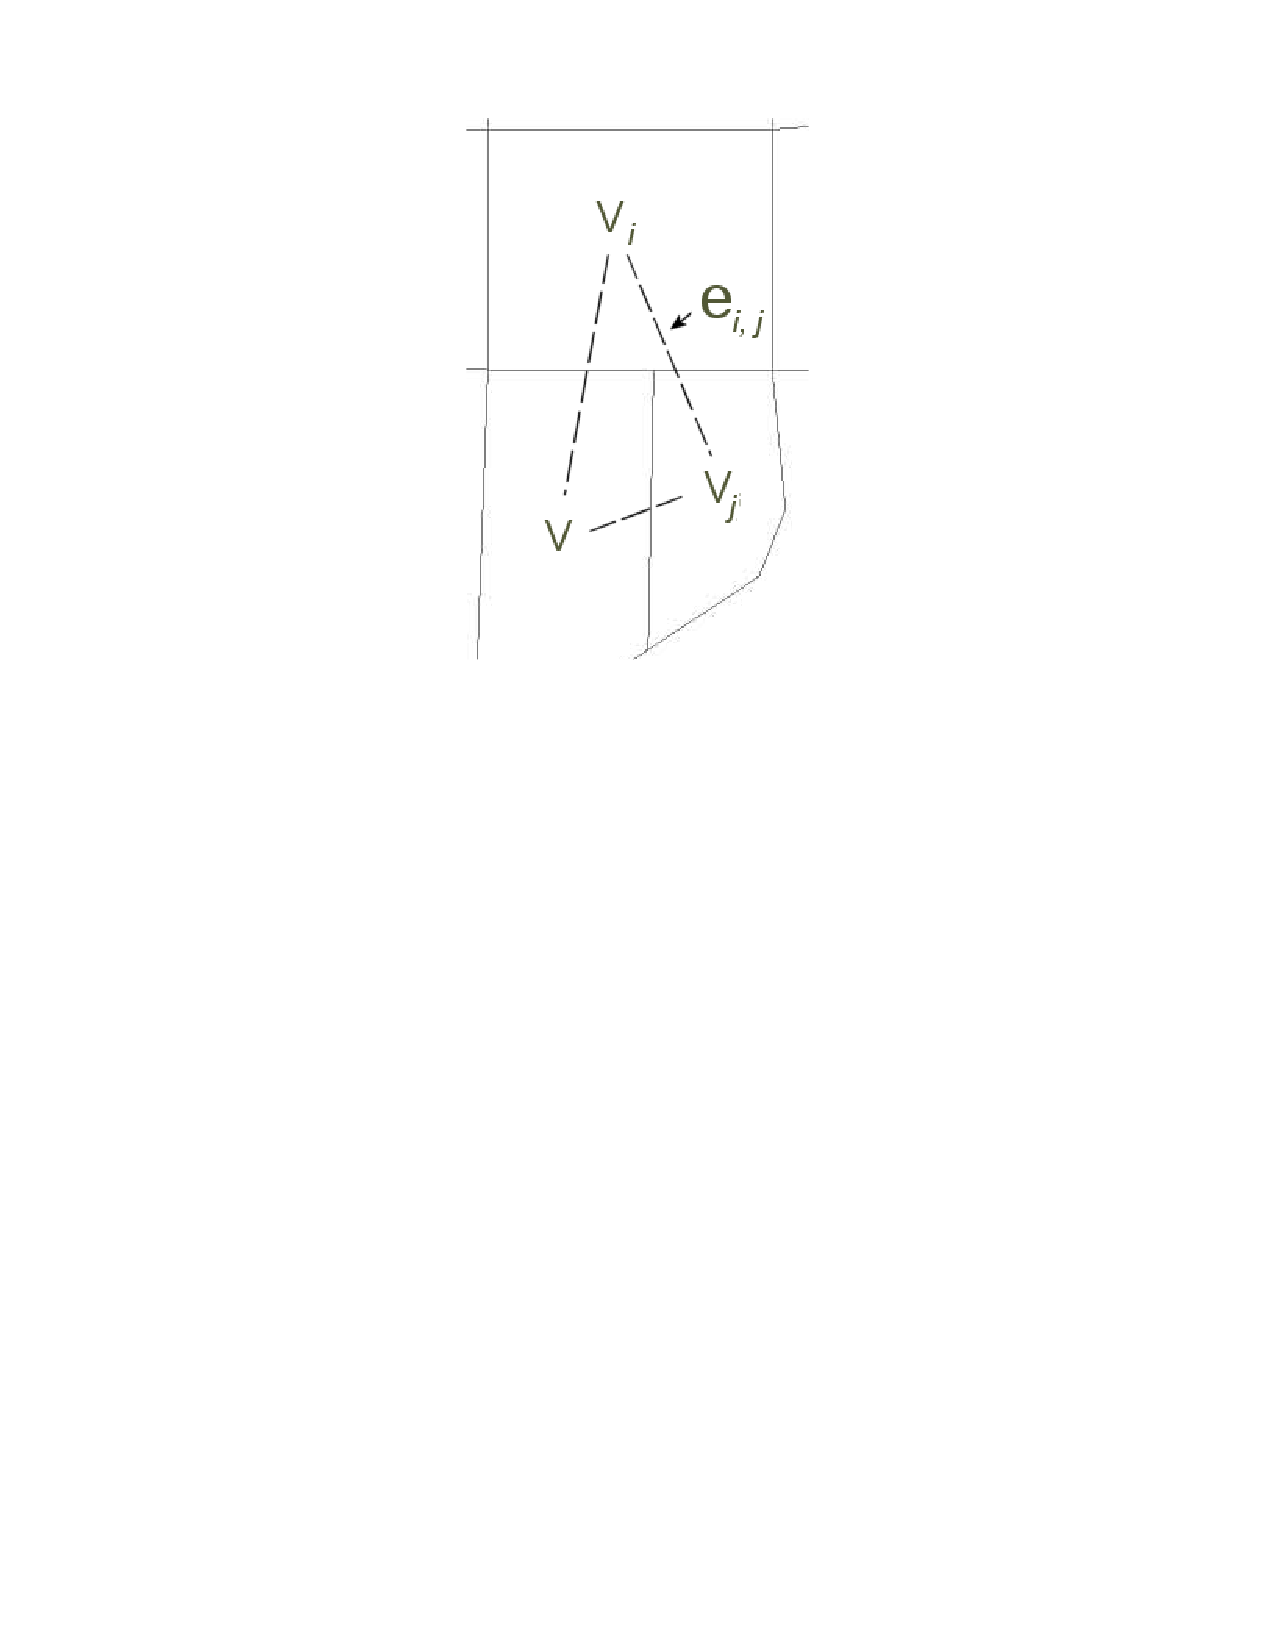
\includegraphics[width=3.5in]{fig_example.pdf}
  \end{center}

  \caption{\small Illustration of redistricting as a graph problem.}
  \label{fig-example}
\end{figure}

Finding an equipopulous, contiguous plan is then equivalent to the following optimization problem, known as
``\textbf{Cut into Connected Components of Bounded Weight''}\citep[see][]{Altman97}: 

Is there a partition of vertices, \textbf{V,}\textit{ }into disjoint
sets \textbf{V}\textit{\textsubscript{1 }}and
\textbf{V}\textit{\textsubscript{2}} such that 
% MathType!MTEF!2!1!+-
% feqaeaartrvr0aaatCvAUfeBSjuyZL2yd9gzLbvyNv2CaerbuLwBLn
% hiov2DGi1BTfMBaeXatLxBI9gBaebbnrfifHhDYfgasaacH8srps0l
% bbf9q8WrFfeuY-Hhbbf9v8qqaqFr0xc9pk0xbba9q8WqFfea0-yr0R
% Yxir-Jbba9q8aq0-yq-He9q8qqQ8frFve9Fve9Ff0dmeaabaqaciGa
% caGaaeqabaaaamaaaOqaamaaqafabaGaae4CamaabmaabaGaamODaa
% GaayjkaiaawMcaaaWcbaGaamODaiabgIGiolaahAfadaWgaaadbaGa
% amymaaqabaaaleqaniabggHiLdGccqGHKjYOcaWGlbaaaa!3E1C!
\[
\sum\limits_{v \in {\bf V}_1 } {{\rm s}\left( v \right)}  \le K
\]
 and 
% MathType!MTEF!2!1!+-
% feqaeaartrvr0aaatCvAUfeBSjuyZL2yd9gzLbvyNv2CaerbuLwBLn
% hiov2DGi1BTfMBaeXatLxBI9gBaebbnrfifHhDYfgasaacH8srps0l
% bbf9q8WrFfeuY-Hhbbf9v8qqaqFr0xc9pk0xbba9q8WqFfea0-yr0R
% Yxir-Jbba9q8aq0-yq-He9q8qqQ8frFve9Fve9Ff0dmeaabaqaciGa
% caGaaeqabaaaamaaaOqaamaaqafabaGaae4CamaabmaabaGaamODaa
% GaayjkaiaawMcaaaWcbaGaamODaiabgIGiolaahAfadaWgaaadbaGa
% aGOmaaqabaaaleqaniabggHiLdGccqGHKjYOcaWGlbaaaa!3E22!
\[
\sum\limits_{v \in {\bf V}_2 } {{\rm s}\left( v \right)}  \le K
\]
and both
\textbf{V}\textit{\textsubscript{1 }}and
\textbf{V}\textit{\textsubscript{2}} induce connected subgraphs of
\textbf{G}\textit{?}



\subsection{Computational  Challenges} 

Formally, redistricting is a computationally complex optimization 
problem \citep[][]{Altman97}.  Perhaps the optimal plan could simply 
be selected by drawing all feasible redistricting plans.  
Unfortunately, for the task of redistricting a state's congressional 
or state legislative districts, no algorithm is guaranteed success 
in a reasonable time.  Consider a modest sized state such as 
Wisconsin, which has slightly more than 330,000 census blocks.  If 
blocks were of equal population, then there would be more possible redistricting plans than there are quarks in the universe.  
More specifically, the number of
possible districts for a given number of blocks and districts is a Stirling Number of the Second Kind:

% MathType!MTEF!2!1!+-
% feqaeaartrvr0aaatCvAUfeBSjuyZL2yd9gzLbvyNv2CaerbuLwBLn
% hiov2DGi1BTfMBaeXatLxBI9gBaebbnrfifHhDYfgasaacH8srps0l
% bbf9q8WrFfeuY-Hhbbf9v8qqaqFr0xc9pk0xbba9q8WqFfea0-yr0R
% Yxir-Jbba9q8aq0-yq-He9q8qqQ8frFve9Fve9Ff0dmeaabaqaciGa
% caGaaeqabaaaamaaaOqaaiaadofadaqadaqaaiaad6gacaGGSaGaam
% OCaaGaayjkaiaawMcaaiabg2da9maalaaabaGaaGymaaqaaiaadkha
% caGGHaaaamaaqahabaWaamWaaeaadaqadaqaaiabgkHiTiaaigdaai
% aawIcacaGLPaaadaahaaWcbeqaaiaadkhaaaGcdaqadaqaaiaadkha
% cqGHsislcaWGPbaacaGLOaGaayzkaaWaaWbaaSqabeaacaWGUbaaaO
% WaaSaaaeaacaWGYbGaaiyiaaqaamaabmaabaGaamOCaiabgkHiTiaa
% dMgaaiaawIcacaGLPaaacaGGHaGaamyAaiaacgcaaaaacaGLBbGaay
% zxaaaaleaacaWGPbGaeyypa0JaaGimaaqaaiaadkhaa0GaeyyeIuoa
% aaa!5408!
\[
S\left( {n,r} \right) = \frac{1}{{r!}}\sum\limits_{i = 0}^r {\left[ {\left( { - 1} \right)^r \left( {r - i} \right)^n \frac{{r!}}{{\left( {r - i} \right)!i!}}} \right]} 
\]


The staggeringly 
large number of plans is actually an underestimate since blocks do not have equal 
population and hence each district might contain a different number of blocks.  Enumeration of all districts with 41,250 blocks would 
further require drawing equal population districts with 
$41,250\pm\epsilon$ blocks.  In practice, contiguity will reduce the number of feasible plans that must be enumerated, 
however, the number of possible plans is still likely to remain staggering.  Thus, selecting the global optimal plan 
from a full enumeration of all plans is not feasible even using the 
fastest computers currently available.

Lacking enumeration, some sort of heuristic is needed to find an 
optimal redistricting plan.  Perhaps an optimal plan can be selected 
from a large number of random plans ``sampled'' from the feasible 
space of redistricting plans. Unfortunately, random assignment of 
blocks to districts will often violate equal population and will 
furthermore violate other criteria, such as contiguity.  An 
algorithm that simply assigns blocks randomly to districts would be 
enormously inefficient as it would produce illegal plans with a high 
probability.  As a consequence, a representative ``sample'' would 
still take a prohibitively long time to draw.

A variant on simple random block assignment is a ``greedy'' 
heuristic that starts from a seed block and randomly assigns 
additional contiguous blocks to a district until a target population 
value is reached.  The advantage of such heuristics is that they 
produce contiguous plans, and have thus been touted as producing a 
random sample of feasible districting plans 
\citep[e.g.,][]{CirDarOro00}.  However, as Knuth warns, just 
because an algorithm is stochastic and appears to behave unpredictably does not mean 
that it produces a true random sample \citep[][]{Knuth97}.  Upon reflection, 
heuristics such as these have a tendency to draw compact districts, since they grow snake-like district boundary tendrils 
with low probability. Thus, greedy heuristics do not randomly sample from the set of feasible redistricting plans and 
might fail to create a near-optimal plan even if run a large number 
of times.

Perhaps a greedy algorithm could find an optimal redistricting plan 
if it selected blocks using a greedy optimization algorithm 
to increase a more general objective function.  Upon reflection, this will 
not work either.  For example, imagine a 
state must draw a district with more than a majority percentage of 
minorities (so called ``minority-majority'' districts) to be in 
compliance with the Voting Rights Act.  Imagine that there are two 
sizable minority communities in a state separated by a white 
suburb.  The only feasible minority-majority district is one that 
links the communities by a narrow bridge across the suburb.  A 
greedy algorithm aimed towards maximizing district minority 
population might easily miss this arrangement because it would reject 
drawing the bridge.  

Furthermore, districts cannot be drawn in isolation from one 
another.  For example, suppose that two minority-majority districts 
were needed to be in compliance with the Voting Rights Act and the 
optimal plan was one that divided the larger of two minority 
communities.  A greedy algorithm might again fail because it would 
not orient the first district in such a manner as to permit the 
creation of the second minority-majority districts (e.g., the first district is composed entirely of the core of the minority community).

As might be expected from the theoretical computational complexity 
of the problems, exact (optimal) methods have been 
unsuccessful in yielding solutions to problems of significant size. 
The most successful of the exact solution methods, based on 
integer-programming formulations, have advanced considerably over 
the last decade, but are still limited to relatively small problems: 
In a recent study a redistricting problem on a 30x30 grid was solved  
\citep[][]{AerEisHeu03} for a fixed set of redistricting 
criteria, and the authors speculated that such methods could be 
extended up to a 50x50 grid. 

Exact solution methods are difficult or impossible to extend to 
arbitrary redistricting criteria. Even integer programming, which is 
one of the most (if not the most) general formulations for which 
exact solution methods are used, requires extensive expertise to reformulate 
redistricting criteria as integer partition constraints.  In contrast, success 
using evolutionary algorithms. on artificial grid data of up to 
500x500 has been reported for a related site-search allocation 
problem \citep[][]{Xiao06}.

\subsection{Available Working Software}

Despite the long history of experiments in automated redistricting, 
there are few tools publicly available for automated redistricting. 
To our knowledge, five commercial software tools produced by Caliper 
Corporation, ESRI, Digital Engineering Corporation (which provides 
a redistricting add-on for ESRI's GIS program), Corona Solutions, 
and Manifold Systems provide automated redistricting functionality 
\citep[][]{AltMacMcD05}.  \footnote{In addition to these companies, 
the Texas Legislative Council developed prior to the 2001 round of redistricting a promising in-house 
automated redistricting program known as TARGET with limited exploratory
capabilities.}   

All of the publicly available tools are limited in several regards.  
First, they are capable only of producing districts with equal 
population and have no means to accommodate other criteria necessary 
to produce legal plans.  All but one program uses variations on 
steepest ascent heuristics, the exception is Corona Solutions which 
claims to uses a single-criterion genetic algorithm.  Unfortunately, we do not know 
much about the internal workings of these programs since they are 
closed source and their algorithmic details pooly documented documented (which raises transparency issues 
similar to the controversies surrounding electronic voting machines).  
As the basic reditricting GIS programs typically cost several thousand dollars (Manifold being the single notable exception), many public interest groups are priced out of redistricting.  

In our testing of these programs, we found that they could generate 
plans automatically, but that these would not be considered legal plans.  
For example, ESRI's automated redistricting algorithm stops growing districts when the 
growing circular districts touch, yielding polka-dot districts that leave much of a state 
unassigned to any district.  Manifold's algorithm apparently grows districts around single seed blocks, sometimes producing a single-block district when other districts are first grown around it.  We do not 
necessarily fault these companies for their rudimentary algorithms.  
There is little \emph{market} demand for automated functionality as 
well-funded redistricting authorities and consultants are reticent to hand over highly sensitive political decisions to a machine.

Furthermore, most experimental work, because it focuses on eliminating politics 
from redistricting (which we believe to be quixotic) implements 
heuristics designed to satisfy compactness, contiguity, and equal 
population (and much of it often takes an ad-hoc view of compactness).  
To our knowledge none looked at either maximizing partisan advantage 
nor competitiveness-- which makes it impossible to use commercial software to 
examine the trade-offs among these potential goals.

\subsection{New Computational Approaches} 

A more general optimization heuristic is needed. In order to be adaptable to any
reasonable redistricting goal, a successful approach should consider not only additions 
of single blocks to a district core, but arbitrary exchanges of multiple blocks among districts.  
To avoid being trapped in local optima, such  a heuristic must be permitted to make 
some backwards (non-improving) steps in search of 
the global optimum, such as bridging two minority communities 
through a white community. These features of the redistricting problem suggest that \emph{metaheuristics} may be an effective practical solution.
 
Over the last two and a half decades, a set of new and surprisingly 
effective heuristic approaches to large optimization problems have 
arisen, including simulated annealing, evolutionary optimization 
(including genetic algorithms), iterated local search (including 
greedy randomized adaptive search), ant colony optimization, and 
tabu search.  These approaches, although formulated independently, 
have now been recognized as belonging to a more general \emph{metaheuristic} framework.

Essentially, metaheuristics are a general approach to optimization that involves 
combining a set of basic heuristics that find optima only in a local neighborhood with a 
larger framework for guiding and applying these heuristics 
repeatedly in a large search space (See \citep[][]{BlumRoli03}, for an in-depth 
survey of metaheuristics, and see 
\citep[][and the citations therein]{Altman97, CortonaEtAl99, 
Xiao03} for surveys of other optimization algorithms used to solve the redistricting problem).  
Designing and applying metaheuristics requires dynamically 
balancing between \emph{diversification}  and \emph{intensification}. Diversification involves generating new 
candidate solutions in such a way as to thoroughly explore the solution space. Intensification involves using (implicitly or explicitly) 
the history of candidate solutions that have been previously evaluated to guide the direction of iterative search. 
Diversification is needed to have a high probability of finding the region of solutions that contains an optimal solution 
and intensification is needed to find these solutions in a practical amount of time. 

Heuristics that are now recognized as being forms of metaheuristic include the aforementioned 
simulated annealing, genetic algorithms, tabu search, and ant colony optimization heuristics, as well as
many more.  All have many variants and parameterizations, and none work well for all optimization problems \citep[][]{WolMac97}.  
Finding the right solution approach for a particular domain of problems is a matter of craft as much as science.

Although no single metaheuristic is guaranteed to be ideal, there are many reasons 
why the metaheuristic framework is an appropriate one to use for approaching redistricting:
\begin{enumerate}
\item First, metaheuristics have a track record of being successful on difficult combinatoric optimization problems. Redistricting is an exemplar of such a problem -- no sure solutions are available and no sure solutions are likely to be discovered due to the problem's computational complexity.
\item Second, in experimental work the heuristics that have been most successful for redistricting-like partitioning problems are forms of metaheuristics.
\item Third, metaheuristics do not assume \emph{a-priori} a set of particular redistricting goals, or operationalization of them (Although 
it is still likely that a particular configuration of selected metaheuristic is better at optimizing on one
type of goal, such as compactness, than another, such as competitiveness). 
By using a general metaheuristic framework we can allow the redistricting plan's author 
the flexibility to specify goals to be satisified, rather than hard-coding the
goals into the the solution method.
\item Fourth, by using multiple metaheuristics to ``solve'' the same problem, 
we reduce the threat that a particular heuristics can 
systematically interact with a redistricting goal \citep[See][]{Altman98} to bias the resulting plan.
\end{enumerate}

Of course, we do not know what the world will be like when fully functional 
automated redistricting software capable of producing legal maps are available.  
Our goal is to produce such software and make it open source and freely available.  
We envision public interest groups would be enabled to draw and actively lobby for their maps; 
courts would no longer necessarily need to adjudicate only between 
maps offered to them by the political parties during litigation; 
academic scholars (and expert witnesses) could use the program to 
explore hypothetical scenarios to test the motivations and outcomes 
of redistricting; and perhaps even politicians would 
be interested in the software as means to remove politics from the 
process.  

The challenge is to develop software that can simultaneously optimize multiple 
criteria and produce legal maps.  Such software must also be flexible 
enough to satisfy differing criteria among the several states.  
Ideally, the software would permit weighting of the criteria in the 
objective function.  To make the program politically feasible, it 
must also be capable of avoiding ``second-order bias'' 
\citep[][]{Parker90}, that is, cleverly selecting criteria to produce 
a favorable political outcome.  Thus, it must also be capable of 
analyzing (and even incorporating into the criteria being optimized) political 
characteristics.

\section {BARD's Modular Approach to redistricting}

The BARD system is divided into separate independent modules in order to facilitate
maintenance and flexibility. Separate modules handle  file input/output, visualization
of plans, computing each family of related scores, and each family of optimization heuristics.

Our approach divides the redistricting process into four independent phases.

The first phase comprises all initialization and configuration.  The user selects the 
geography to load along with any demographic and political variables and selects 
the set of metaheuristics to apply. The user also configures the formula used to 
evaluate the plan. Typically, this formula is a weighted combination 
of equal population, target racial population, compactness, geographic constraints, 
and election data for predictive election outcomes. We
supply these and many other ``building block'' scores in BARD and users can write 
their own scores as well, using any function supplied in \proglang{R} and any combination
of demographic or geographic variables they supply with their maps. 

The second phase comprises the generation of \emph{starting points} for redistricting plans.
The user may choose to start from pre-existing plans (e.g. chosen by the legislature, or offered
by a public interest group) if available, or to have BARD generate arbitrary plans using 
random assignments, random walks, or other stochastic procedures.

The third phase, applies the metaheuristics and cost function configured in phase one to the 
starting points generated in phase two. This involves significant computation and should yield a plan that is
(at least) a local optimum for the given scoring formula. 

The second and third phases are repeated, possibly while varying the weighting of components of the score formula, 
to generate a set of plans. The resulting plans vary over the 
values of the individual score components and overall score (either due to the systematic 
reweighting of score components, or due to the variance among starting points).  

In phase four, the set of candidate plans is analyzed. BARD outputs the 
range of overall scores, the range of scores for each component, the differences 
among plans, and the correlations among score components.  Candidate plans 
may also be contrasted with the starting plans if meaningful pre-existing starting 
points were selected.  This analysis phase can thus reveal the trade-offs among
redistricting criteria between a starting map and an optimized map.

\subsection{Optimization Details}

The initial version of BARD includes both \emph{simulated annealing} and \emph{genetic algorithms} 
as optimization metaheuristics. As \citep[][chapter 4]{AltGilMcD03} explains:

%TODO: Paraphrase/daspt
\emph{Simulated Annealing} (SA) exploits an analogy between the
way in which molten metal freezes into a minimum energy
crystalline structure (the annealing process) and the search for a
function optimum.   At each iteration, simulated annealing randomly generates
a candidate point (or set of points) within a local neighborhood
of the current solution. The probability of moving from the
current solution to one of the candidate points is a function of both
the difference in the value of the objective function at each point, and a 
temperature parameter. At high temperatures, candidate points that are ``worse'' than 
the current solution can be selected as the solution in the next iterate.  This helps the 
heuristic to avoid a local optimum. At each iteration, the temperature is reduced gradually, so 
that the probability of heading downhill becomes vanishingly small.

\emph{Genetic Algorithms} (GA) are a form of heuristic inspired by analogies 
between optimization (and adaptation) and the evolution of competing
genes.  In a genetic algorithm, a population set of candidate solutions are supplied to the optimization problem. 
Each solution is encoded as a string of values. At each iteration each member of the population is subject, at random, 
to mutation (an alteration of the solution vector), hybridization (a reshuffling of subsequences between two solutions). 
In addition, each round undergoes selection, where some solutions are discarded, and some are 
duplicated within the population, depending on the fitness (function evaluation) of that member.

Solving difficult optimization problems, however, is as much an art as a science.  
BARD incorporates many optimizations such as dynamically updating
scores based only on the parts of districts that changed, and use of optimized ``C'' code
to supplement the main \proglang{R} framework.

Optimization algorithm performance can be quite sensitive to starting values when a function has
multiple local optima.  The redistricting problem is rife with local optima.  In practice, optimization algorithms 
can frequently become trapped in a local optima. This is true even for metaheuristics, 
unless the metaheuristic can adapt (or is adpated by the researcher to) the particular problem.  

Part of the difficulty lies in trying to optimize on multiple constraints, for example the case of equal population and contiguity.  
A solution that scores well on equal population may have difficulty improving to create a map with contiguous districts. 
Or, a map that is contiguous may have difficulty improving to create a map that has more equal population among districts. 

Another part of the difficulty has to do with the size of the local neighborhood being searched at each iteration.  
Sometimes an algorithm must take large steps to escape the basin of attraction that leads back to a local optima. 
For example, a simulated annealing algorithm that considered only a single trade of census blocks among districts at each iteraction 
may become trapped in a local optima more easily than one that considers trades of two or more blocks at a time.  
	
Selecting good starting values makes it much easier for metaheuristics to yield improved plans.  
In practice, when one starts with a current legal plan, it is much faster to generate a new, better-scoring plan 
than when starting from an entirely random district.  The problem with using the former districts as a starting point is that 
political motivations that predominate the district shapes will continue to influence the solution.  In some cases, we would 
like to entertain solutions that are potentially far from the former districts.

We have implemented three types of algorithms to produce district starting seeds.  The first is a simple random 
assignment of geography to districts, which we implement to create districts that are near to equal population but 
have a small probability of being contiguous.  Another algorithm, which we call \emph{k}-means, creates \emph{n} districts from a \emph{n}-number 
of random seeds by assigning all bits of geography based on the closest seed centroid to the geography's centroid.  \emph{K}-means tends to produce 
nearly-contiguous (and relatively compact) districts that are of unequal population.  A third algorithm is a greedy algorithm that 
grows districts from seed values and builds districts by assigning geography that best improve 
on the score function.  The greedy algorithm can produce contiguous equal population districts, 
but tends to draw elongated districts, can get stuck, and is computationally intensive.
	
We have experimented most with optimization using districts generated by 
random assignment and \emph{k}-means.  We have found these starting maps tend to be 
extremes on the two dimensions, scoring well on equal population or contiguity, but not both.  Our optimization algorithm 
evaluates trades of a single geography between districts.  As such, we find that the optimization algorithm 
has difficulty displacing itself from the local optima to one that scores well on both equal population and contiguity.
	
A solution we are exploring is to dynamically aggregate selected blocks to speed computations.  We are 
experimenting with two solutions, one considers trades of aggregate geography, such as counties rather than census blocks.  
The other considers a trade of a random point and all geography in the closest path from the point to the candidate district.  
These solutions are promising, but as to date have yet to solve our problems.  The aggregate geography approach has led us to 
re-evaluate implementation of the greedy starting-seed algorithm, as it may be possible to develop 
a less-computationally intensive greedy algorithm that is at the same time ``smart'' in that it uses the k-means algorithm to 
draw relatively compact districts. 

%Discuss other crucial algorithms involved: efficient updates of value functions,
%dynamic adjustments of units of aggregation, computing bounds for value functions 
%-- value function evaluation ordering, particularly difficult value functions.
%
%Discuss crucial implementation issues: tuning parameters, numerical issues.
%
%Cacheing previous calculatiosn, avoid recalculating things that have not changed, incremental
%recalculation, plans. 

\section{Plan evaluation and exploration}

A unique aspect of BARD's approach is that it enables
one to explore the tradeoffs between redistricting goals, such as the
de{}-minimis population inequality effect and district
compactness, the creation of an additional majority{}-minority
district and the number of partisan seats, and district
competitiveness and compactness. We can repeatedly
generate plans using the same set of redistricting goals,
while systematically changing the weight given to
one (or two) of those goals, and then examine systematic trends in
plan scores in one more dimensions. For example, if plans that are generated
using a scoring rule that weights compactness heavily have
significantly fewer minority districts than plans generated with a
lower weight on compactness, this suggests a tradeoff exists
between compactness and minority representation.

A variant of this technique can also be applied to reveal the
preferences of those who created a districting plan. Informally, if we
start with a redistricting plan chosen by a set of participants and
show that a small modification to this plan has a large impact on 
a particular goal, we can infer that the author of the plan places a low
value on that goal. For example, if one can make plan more competitive, at the expense
of a small degree of compactness, while keeping the plan the same in all other
relevant ways, then we have reason to believe that the author of the plan 
valued compactness over competitiveness. 

Courts and litigants have used this approach informally, especially in the
absence of smoking gun evidence, when they examine characteristics of
plans that were rejected to illuminate why a particular plan was
accepted. For example, it has been used by academics to assess
intent in North Carolina's redistricting in the 1990s \citep[][]{GronWil99}. Using automated redistricting it is possible to
systematize this method -- BARD facilitates this. 

Formally, this technique based on a fundamental axiom in economics, the Weak Axiom
of Revealed Preference (WARP) \citep[][]{Samuelson48}. Any method to infer preferences
from the actions of a rational actor must rest on WARP.  WARP states
that if one observes a choice 
% MathType!MTEF!2!1!+-
% feqaeaartrvr0aaatCvAUfeBSjuyZL2yd9gzLbvyNv2CaerbuLwBLn
% hiov2DGi1BTfMBaeXatLxBI9gBaebbnrfifHhDYfgasaacH8srps0l
% bbf9q8WrFfeuY-Hhbbf9v8qqaqFr0xc9pk0xbba9q8WqFfea0-yr0R
% Yxir-Jbba9q8aq0-yq-He9q8qqQ8frFve9Fve9Ff0dmeaabaqaciGa
% caGaaeqabaaaamaaaOqaamaacmaabaGaamyyaaGaay5Eaiaaw2haaa
% aa!34BB!
\[
\left\{ a \right\}
\]
 from a set 
% MathType!MTEF!2!1!+-
% feqaeaartrvr0aaatCvAUfeBSjuyZL2yd9gzLbvyNv2CaerbuLwBLn
% hiov2DGi1BTfMBaeXatLxBI9gBaebbnrfifHhDYfgasaacH8srps0l
% bbf9q8WrFfeuY-Hhbbf9v8qqaqFr0xc9pk0xbba9q8WqFfea0-yr0R
% Yxir-Jbba9q8aq0-yq-He9q8qqQ8frFve9Fve9Ff0dmeaabaqaciGa
% caGaaeqabaaaamaaaOqaamaacmaabaGaamyyaiaacYcacaWGIbGaai
% ilaiaadogaaiaawUhacaGL9baaaaa!37EA!
\[
\left\{ {a,b,c} \right\}
\]
  then it must be the case that
% MathType!MTEF!2!1!+-
% feqaeaartrvr0aaatCvAUfeBSjuyZL2yd9gzLbvyNv2CaerbuLwBLn
% hiov2DGi1BTfMBaeXatLxBI9gBaebbnrfifHhDYfgasaacH8srps0l
% bbf9q8WrFfeuY-Hhbbf9v8qqaqFr0xc9pk0xbba9q8WqFfea0-yr0R
% Yxir-Jbba9q8aq0-yq-He9q8qqQ8frFve9Fve9Ff0dmeaabaqaciGa
% caGaaeqabaaaamaaaOqaaiaadggacqGHLjYScaWGIbGaaiilaiaadg
% gacqGHLjYScaWGJbaaaa!397B!
\[
a \ge b,a \ge c
\]
To illustrate with a simple example, WARP implies that if I like
chocolate ice cream over vanilla and strawberry, I will choose
chocolate when presented with either a choice between chocolate and
vanilla or chocolate and strawberry. 

In a redistricting context, if plans \textit{a} and \textit{b} are available, but 
plan \textit{a} is
chosen, than it must be that plan \textit{a} is weakly preferred.
\ Using this method to reject competing hypotheses does \textit{not}
require the distributional assumptions that limit sampling heuristics.
\ WARP is deterministic: the probability that \textit{b }{\textgreater}
\textit{a} when \textit{a} is chosen, equals zero.\footnote{\ Any
method for inferring intent must assume some weak collective
rationality -- that what is intended is also what is chosen. If this
assumption is violated, and the preferred plan is not the one chosen
(at least probabilistically), then any attempt to infer intent is
futile.}

We can use computationally intensive district generation techniques 
to reveal intent using WARP.  The optimization algorithm can  
map out the space of local optimum of a value function that captures all relevant 
redistricting goals.  For example, if there exists a plan that contains one more 
minority district than an adopted map, and there is no difference in terms of other
geographic and political goals, then maximization of minority districts was not a 
goal of a redistricting authority.

A limitation of this approach is that a redistricting authority must be reasonably aware
of the existance of an alternative map.  In some states, maps revealed through 
public submission phases of a redistricting process can help chart a redistricting authority's preference
structure.  Where public submissions are not permitted, optimization from the starting seed of the 
adopted map may reveal if there was an easily discoverable district configuration that would have improved
a map on a given criterion under study.

There are three further limitations to this approach.  First, the choice of \textbf{K},\textbf{ I},\textbf{
}and\textbf{ R} should represent plausible explanations of the goals of
the redistricting process in the political context being analyzed: Like
any other statistical test, a set of reasonable causal hypotheses must
be a starting point. \ \ Second, like any other analytic method, its
effectiveness will depend on how informative the data is. In some cases
it may fail to reject any of the competing hypotheses, and one may need
to obtain more data, such as other plans that were under consideration.
Finally, to be interpreted as revealing \textit{preference
}\textup{\ rather than simply }\textit{opportunity }plans used for
comparison must have been reasonably discoverable by a redistricting
authority. However, since this method uses real plans as a starting
point, our method requires \ only that a districting authority be aware
only of plans that were directly related to proposed plans, while most
statistical methods of analyzing plan choice assume that the
districting authority was aware of, and had a choice over, of the
\textit{entire distribution }of plans.

\section[How to use BARD]{How to use \pkg{BARD}}

This brief example shows how BARD can be used: 



\begin{Schunk}
\begin{Sinput}
> packageDescription("BARD")
\end{Sinput}
\end{Schunk}

This shows the initial geography being loaded, and random starting point plans created and plotted:
\begin{Schunk}
\begin{Sinput}
> brown.map <- bardImportShape(system.file("shapefiles/Brown_block.shp", 
+     package = "BARD"), galfile = system.file("shapefiles/Brown_block.GAL", 
+     package = "BARD"))
> ndists <- 5
> kplan1 <- kmeansPlan(brown.map, ndists)
> kplan2 <- kmeansPlan(brown.map, ndists)
> rplan <- randomPlan(brown.map, ndists)
> cplan <- CDOcontiguityPlan(brown.map, ndists, usebb = TRUE)
> op <- par(ask = TRUE)
> plotPlan(kplan1, brown.map)
> plotPlan(kplan2, brown.map)
> plotPlan(rplan, brown.map)
> par(op)
\end{Sinput}
\end{Schunk}

This is a comparison of the starting plans:

\begin{Schunk}
\begin{Sinput}
> comparePlans(list(kplan1, kplan2, rplan), brown.map, scores = list(Pop1 = score1, 
+     Pop2 = score2))
\end{Sinput}
\end{Schunk}

This shows the cost function configuration, and optimization phase:

\begin{Schunk}
\begin{Sinput}
> funcs <- c(pop.bw, pop.mean.var)
> b.vars <- c("POP", "POP")
> var.weight <- c(1, 1)
> optim.env = new.env()
> scoreGenerator <- costWrapper(func.family = funcs, block.vars = b.vars, 
+     dataframe = brown.map$shape$att.data, baseMap = brown.map, 
+     ndists = 5, weight = var.weight)
> score1 <- function(plan, basemap) {
+     scoreGenerator(plan, resetScore = TRUE)
+     return(pop.bw(dataframe = brown.map$shape$att.data, baseMap = basemap, 
+         ndists = 5))
+ }
> score2 <- function(plan, basemap) {
+     scoreGenerator(plan, resetScore = TRUE)
+     return(pop.mean.var(dataframe = brown.map$shape$att.data, 
+         baseMap = basemap, ndists = 5))
+ }
\end{Sinput}
\end{Schunk}




\begin{Schunk}
\begin{Sinput}
> funcs <- c(pop.mean.var, pop.bw, pop.max.dev, compact.REOCK, 
+     scoreContiguity)
> b.vars <- c("POP", "POP", "POP", "NULL", "NULL")
> var.weight <- c(2, 2, 1, 1, 2)
> optim.env = new.env()
> mymap <- function(plan, ...) {
+     plotPlan(plan, brown.map$polys, ndists, ...)
+ }
> myscoreO <- costWrapper(func.family = funcs, block.vars = b.vars, 
+     dataframe = brown.map$shape$att.data, baseMap = brown.map, 
+     ndists = 5, weight = var.weight)
> gp2 <- optimGenWrapper(genPlanR, basemap = brown.map, onewayprob = 0.2, 
+     plotf = NULL, DEBUG = TRUE)
> system.time({
+     plan1a <- optim(round(kplan1), myscoreO, gr = gp2, method = "SANN", 
+         control = c(maxit = 1000, temp = 10, tmax = 1))
+ })
> myscoreO(plan1a$par)
> mymap(plan1a$par)
\end{Sinput}
\end{Schunk}



\section{Summary}


BARD is still in early release. However, even in its current state, it is the only open-source redistricting system available.  Moreover, BARD is the only publicly available (commercial or non-commercial) software that does multi-criteria optimization, allowing the user to specify a formula that includes more than one variable.  Finally, BARD is  unique in providing  a framework for the systematic analysis of tradeoffs in redistricting 


Our package can be obtained from the project website \url{bard.sf.net}, any CRAN mirror (\url{http://cran.r-project.org/}).
 
\section{Acknowledgements}\vspace{-5pt}

We thank Max Tsvetovat and Mike Margolis for their comments and recommendations, and Mark Rouleau for research assistance and programming.  Turning to institutional sponsors, we thank the Joyce foundation for its support, without which this research would have been impeded. 

\section{References}\vspace{-5pt}
\bibliography{bardJSS}
\end{document}
